\chapter{Evaluation}
\label{chap:Evaluation}
\renewcommand{\arraystretch}{0.5}

In this chapter, we will go through our experimental hypotheses, testing scenarios, experiments conducted on two sample 
stereo matching algorithms, SGBM and ADCensusB, and the results with our
proposed evaluation system to assess the benefits of using our evaluation model for outdoor AR applications over the general-purpose evaluation models; 
the Middlebury and Kitti Stereo Evaluation.

\section{Stereo Dataset}
It should be noted that the stereo images we have used to conduct the experiments on stereo algorithms in our system,
are selected from the Kitti Stereo Dataset.
In contrary to the Middlebury dataset, the Kitti Stereo Project provides stereo images and ground truth disparity maps
that are taken from outdoor scenes under real circumstances. These properties them more appropriate 
for evaluating the performance of the algorithms in outdoor AR applications, thus better meeting the objectives of this study.
We have selected fifty-two image pairs from the Kitti Stereo dataset based on different photometric and visual properties that are important
in stereo vision and an AR application, as observed by the human visual system. Some 
of these properties are listed as follows:
\begin{itemize}
\item Variation in light and shading, that is, the scenes including bright, dim, and dark regions.
\item Various depth ranges, that is, including near field, medium field and far field objects. 
\item Various degrees of depth discontinuity and occlusion, as observed in the images.
\item Well textured and not properly textured regions.
\end{itemize}

\section{Methodology}

Before going through the explanation of the experiments to assess our evaluation model, we restate our main research question in this
study to better justify our hypotheses and the experiments defined for their validation. 
As mentioned earlier in Chapter \ref{chap:Introduction}, our main objective is to investigate whether using 
stereo matching techniques to generate the depth map of the 
surrounding environment in an outdoor AR application can meet the requirements of the AR system. 
Therefore, our experiments focus 
on assessing those aspects of our evaluation model that assist to better answer this question.
As a result, our first attempt towards evaluating our model is to investigate and demonstrate whether the results of the evaluation process 
are properly measured and presented in the framework of the important factors in an outdoor AR application.
After confirming this property, which is the key property of our model, we investigate the effect of our proposed masking 
approach on the evaluation results. Moreover, we present how the methods are evaluated in the framework of 
real-time interactive AR systems.
We also explain how the evaluation and comparison of the methods is done in our model with some
experiments on the sample stereo matching algorithms.

\section{Hypotheses}

We have defined a set of hypotheses to evaluate our proposed design. These hypotheses are as follows:

\begin{itemize}
\item \textbf{Hypothesis 1}: \emph{Our model is more suitable than other approaches to evaluate and demonstrate
the performance of the stereo matching algorithm in the framework of 
outdoor augmented reality applications.} 
Unlike the Middlebury and Kitti benchmarks which are considered general-purpose evaluation models, 
our system can particularly evaluate the algorithms in the framework of an 
outdoor augmented reality application to facilitate the process of determining
the proper method for using in the AR system for a high quality real-time generation of the depth map of the surrounding environment from 
the user's point of view.

\item \textbf{Hypothesis 2:} \emph{Observing, evaluating, and consequently 
refining the areas near the depth edges in an image are more important in an AR application.}

Salient edges caused by depth discontinuities, 
which can also represent the object boundaries and occlusion, are one of the 
most important depth cues that helps the observer to better perceive the depth of different objects in the scene. In other words, the areas near the edges corresponding to depth discontinuities
in a scene are more important to the human visual system for perception of depth in an AR application and, therefore, the disparity 
errors in these regions can be detected easier by the HVS. Therefore, we argue that in our model, which has the property of masking and evaluating the results for
these particular regions,
the evaluation results can be of great value to an outdoor AR application.

\item \textbf{Hypothesis 3:} \emph{Our system is better than other evaluation models for assessing the performance of the algorithm in
real-time AR applications.}

Other evaluation models, the Kitti and Middlebury benchmarks, do not evaluate and report on the efficiency of the algorithms
with respect to their execution time. On the other hand, our system is capable of examining and evaluating an algorithm 
based on its execution time and, therefore, can report on its efficiency for real-time AR applications.

\item \textbf{Hypothesis 4:} \emph{The trade-off between the accuracy and the running time of the stereo algorithms can be effectively evaluated 
in the framework of an outdoor AR application through our system.} 

Nearly all the solutions to the problem of stereo correspondence have been dealing with the trade-off between the accuracy of the results and the running time.
Therefore, most of the solutions focus only on improving one of these aspects in the final results. Some methods use certain post processing techniques to refine the 
disparity results in the end, thus improving the accuracy, whereas the others propose particular approaches that can be implemented on the GPU to reduce the processing time.
Due to the importance of both metrics in an outdoor AR application, we argue that the trade-off between these metrics can be effectively analyzed in our evaluation system.

\item \textbf{Hypothesis 5:} \emph{The ability to detect the difference in depth in stereo correspondence methods not only depends on their accuracy
in estimation of the disparity values, but is also affected by other factors, such as the environmental noise, the resolution of the capturing device and its
robustness to noise.}

According to different studies \cite{dras96, kru10,azuma01}, some other factors such as issues associated with the environment, display devices, or capturing devices
can also affect the perception of depth in the visual system. As a result, we hypothesize that the ability to detect the difference in depth in an outdoor AR system,
does not merely depend on the accuracy of the stereo correspondence algorithm, and other factors should also be taken into account.
\end{itemize}
\noindent
The experiments designed to validate these hypotheses are explained in the following sections.

\section{Experimental Environment and Settings}
Experiments were carried out on a Linux machine with Intel Core(TM) i7 3.20GHz CPU. 
Although the GPU-based approach to both algorithms are proposed in the literature,
we have used their CPU implementations in this research, since none of the GPU implementations is publicly available.

The disparity results from our implementation of ADCensus corresponding to Tsukuba and Venus images from Middlebury dataset, 
Figure \ref{fig:midburyimgs}, is shown in Figure \ref{fig:midburydisps}, 
which nearly resemble the results published in the paper \cite{mei11}, presented in Figure \ref{fig:adcmidbury}. 
Since we could not find access to the original disparity images generated by ADCensus to make a solid comparison with our disparity results from ADCensusB, 
we leave it to the reader to judge the similarity between these images. We also provide a brief description of our implementation of 
ADCensusB in Section \ref{subsec:adcB}. \newline
The set of parameters used at different steps of the evaluation are presented in the following sections.
It should be noted that these parameters were kept constant for all the images and experiments. However, if a parameter is changed during an experiment for specific
reasons, it will be explicitly mentioned in the description of the experiment.

\begin{figure}[H]
\centering
\subcaptionbox{Tsukuba image}
[.5\linewidth]{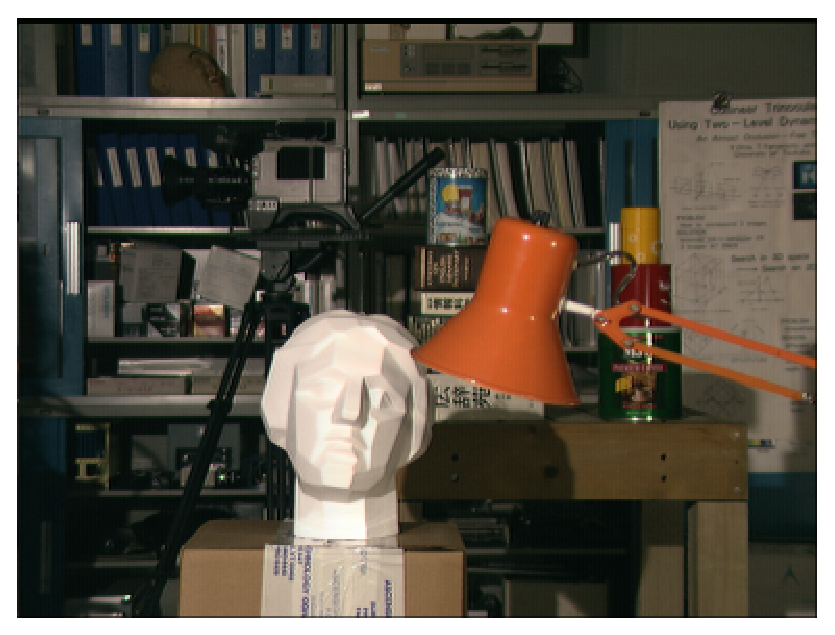
\includegraphics[scale=0.5]{tsukubaL}}%
\subcaptionbox{Venus image}
[.5\linewidth]{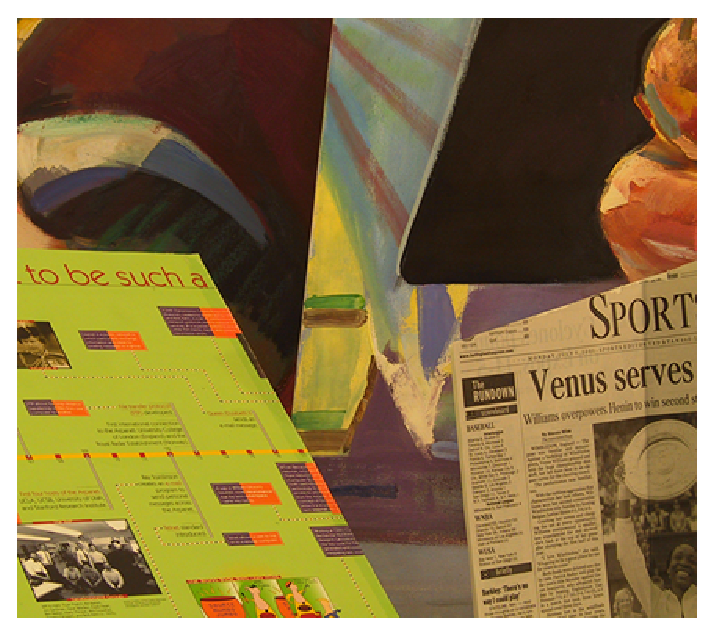
\includegraphics[scale=0.51]{venusL}}%
\caption{Sample images from Middlebury stereo dataset \protect\cite{midbdata}}
\label{fig:midburyimgs}
\end{figure}

\begin{figure}[H]
\centering
\subcaptionbox{Tsukuba disparity image by ADCensus}
[.5\linewidth]{
\includegraphics[scale=0.5]{adctsukuba}}%
\subcaptionbox{Venus disparity image by ADCensus}
[.5\linewidth]{
\includegraphics[scale=0.51]{adcvenus}}%
\caption{Disparity images by ADCensus for Middlebury images in Figure \protect\ref{fig:midburyimgs}}
\label{fig:adcmidbury}
\end{figure}

\begin{figure}[H]
\centering
\subcaptionbox{Tsukuba disparity image by ADCensusB}
[.5\linewidth]{
\includegraphics[scale=0.5]{tsukubadisp}}%
\subcaptionbox{Venus disparity image by ADCensusB}
[.5\linewidth]{
\includegraphics[scale=0.51]{venusdisp}}%
\caption{Disparity images by ADCensusB for Middlebury images in Figure \protect\ref{fig:midburyimgs}}
\label{fig:midburydisps}
\end{figure}

\subsection{ADCensusB Implementation} \label{subsec:adcB}
As thoroughly described in the paper by Mei et al. \cite{mei11}, our implementation includes various cost estimations
at different steps of the algorithm that are computed by separate functions in the code; as a result of each function call, 
specific arrays of type \textit{float} corresponding to various costs are filled in and used by the subsequent functions in the algorithm.
The main cost estimations are as follows:
\begin{enumerate}
\item \textbf{AD-Census Cost:} The initial matching cost which consists of the average intensity of pixel values in the left and right images, 
and the census cost that is formulated
based on the relative ordering of the pixel intensities within a specific window size \cite{hirseval09}, defined as a $9\times7$ window in the implementation. This 
step is accomplished by three function calls in our implementation which are named \textit{costAD}, \textit{c\_census} and \textit{initCost}.
\item \textbf{Aggregated Cost:} The aggregated matching cost of each pixel over a specified support region, which is defined as a cross-based 
region in the paper and originates from the method proposed by Zhang et al. \cite{zha09}. This cost is computed by a function called \textit{aggregatecost}
in our implementation
\item \textbf{Path Cost:} The path cost that is estimated from the aggregated cost of each pixel by scanline optimization from different directions. The idea of
multi-direction cost optimization originates from Hirshmuller's semi-global matching solution \cite{hir08}. This step is accomplished by a function called 
\textit{scanline} in the implementation.
\end{enumerate}

We have followed the approach in each of the referenced papers for the implementation of each cost estimation. As a result of the aforementioned steps
a 3 dimensional cost volume with the size of $image\_width\times image\_height\times disparity\_range $ is generated as the final cost of type \textit{float}.
After this step, disparity values are selected by following the ``winner takes all'' approach, that is, the disparity with the minimum cost is
selected as the final disparity value of each pixel \cite{sch02}.
After the main body of the method is implemented, the algorithm proceeds with a multi-step refining process. This step, which is one of the unique features
of ADCensus method, attempts to detect the outliers, that is the wrong matches of pixels, and refines the disparity results based on the detected outliers.
For the detection of outliers, we follow a common approach  
known as left-right (L-R) consistency check. In this check, the disparity map for both
the left and right images is first calculated. Then, if a pixel in the left image, based on its disparity value, corresponds to a pixel in the right image
that does not map back to it, it will be labeled as an outlier \cite{mei11}. This description can be formulated as follows:

\begin{align}
D_{L}(p) \neq D_{R}(p-(D_{L},0))
\end{align}
\noindent
Where $D_{L}(p)$ is the disparity function for the left image and $D_{R}$ is the disparity function for the right image. \newline 
In our implementation of ADCensus, we have the L-R check and its subsequent refinement steps triggered with a flag.
Therefore, when the flag is not set, neither the check nor the refining steps are triggered in the algorithm.
Following the proposed approach in the paper, we also have multiple steps of refinement in our implementation, which occurs through different function calls.
These functions are as follows:
\begin{enumerate}
\item \textit{findOutliers}, which tends to find the outliers by conducting the L-R check.
\item \textit{regionVoting}, which iteratively updates the disparity value of each outlier pixel 
based on a histogram of its reliable neighboring pixel values in its cross-based support region; the disparity with the most votes in the neighboring region 
is chosen as the final disparity value of the outlier pixel.
\item \textit{interpolate}, which follows an interpolation strategy to find the remaining outliers disparity value based on their 
16 reliable neighboring pixels. 
In this strategy, mismatch pixels are
interpolated differently from occluded pixels. If a pixel is occluded, its disparity is taken from the background, that is, the minimum disparity of its neighboring
pixels is selected as the disparity value of the outlier pixel. On the other hand, if the pixel is a mismatch point, the disparity of the pixel with the most
similar color to the outlier pixel, is selected from the neighbors.
\item \textit{discAdjust}, which first attempts to find the edges in the disparity map, that is, finding the depth discontinuities, and then, for each pixel on any
detected edges, the disparity values of its neighbors on the both sides of the edge are sought. Next, the disparity value of the pixel of interest is updated with the disparity of 
any of the adjacent pixels with the least matching cost.
\item \textit{subpxEnhance}, which applies a quadratic polynomial interpolation on the estimated disparity values to decrease the discretization 
error and is followed by a $3\times3$ median filter for smoothing the results.  
\end{enumerate}
We have attempted to carefully follow and implement the strategies described in ADCensus solution as explained in \cite{mei11}; however, measuring the extent to which
our implementation is close to the proposed method is a matter out of hand, due to unavailability of any actual disparity image 
to compare our results with or the original source code of ADcensus.
It should also be noted that we could not proceed with porting our implementation to GPU due to time constraint and inadequate description
about it in the published paper.

\subsection{Masking}
In order to build the masks in our system, the OpenCV Canny edge detector and Dilation are used.
Canny have been used to detect the depth edges in the ground truth disparity map, and the dilation operation 
for expanding the detected edge regions in the masking process. The extent to which the regions are expanded
is determined by the number of iterations in the dilation operation. Table \ref{tab:candilparam} shows the parameters used in the Dilation
and the Canny edge detection. However, the \textit{minimum threshold} in Canny is tuned and selected separately for each image 
since the threshold should change depending on the scene. \newline

%{\footnotesize
\begin{minipage}{\linewidth}
\begin{center}
\captionof{table}{Masking Parameters}
\label{tab:candilparam}
\begin{tabular}{ |c|c| }
\hline
Dilation\_iterations & 10 \\  \hline
Canny\_apertureSize & 3 \\ \hline
\end{tabular}
\end{center}
\end{minipage} \newline
%}

The ground truth disparity maps in the Kitti stereo dataset are generated by a 3D laser scanner, thereby resembling
a point cloud map of discrete disparity values. This property of the disparity images 
can be problematic for the masking process since it can result in many small streaks as the edges.
Therefore, before applying any edge
detection on the image, we need to first fill the gaps by interpolating the values and obtain a smoothed ground truth disparity.
This can be achieved by applying a dilation operation.
In our implementation, we have used the OpenCV dilation operation with different number of iterations for each image, that is set depending on the scene 
and the original ground truth disparity, to obtain a fully dense disparity map. 
The new disparity images are then stored on the disk for further use.
However, it should be noted that the dilated disparity images are only used in the construction of the edge masks while detecting the depth
edges in the image.
%However, it should be noted that the ground truth disparities used for the related comparisons and calculations 
%in the evaluation process, are the original disparity images before being dilation.

\subsection{Stereo Algorithms Settings}
The parameters for each algorithm used in our experiments to generate the disparity
maps are kept constant over all the images in the dataset. These parameters are presented in Tables \ref{tab:sgbmparams} and \ref{tab:adcparams} 
for SGBM and ADCensusB, respectively. \newline

%{\footnotesize
\begin{minipage}{\linewidth}
\begin{center}
\captionof{table}{SGBM Parameters}
\label{tab:sgbmparams}
\begin{tabular}{ |c|c|c|c|}
\hline
SADWindowSize & 9 & disp12MaxDiff & 2 \\ \hline
uniquenessRatio & 10 & P2 & 3*9 \\ \hline
speckleWindowSize & 100 & speckleRange & 2 \\ \hline
\end{tabular}
\end{center}
\end{minipage} \newline \newline
%}

\noindent
Other parameters not mentioned in the table are considered with their default values. \newline

%{\footnotesize
\begin{minipage}{\linewidth}
\begin{center}
\captionof{table}{ADCensusB Parameters}
\label{tab:adcparams}
\begin{tabular}{|c|c|c|c|c|c|c|c|}
\hline
$\lambda_{AD}$ & 10 & $\lambda_{Census}$ & 30 & $L_{1}$ & 34 & $L_{2}$ & 17 \\ \hline
$\tau_{1}$ & 20 & $\tau_{2}$ & 6 & $\pi_{1}$ & 1.0 & $\pi_{2}$ & 3.0 \\ \hline 
$\tau_{SO}$ & 15 & $\tau_{S}$ & 20 & $\tau_{H}$ & 0.4 & & \\  \hline
\end{tabular}
\end{center}
\end{minipage} \newline \newline
%}

The minimum and maximum disparity values are also kept constant for each image pair in both algorithms; however, the maximum 
disparity differ for each image pair as the scenes are different
and objects are located at different depth fields.
The minimum disparity is set to $0$ for both algorithms. The maximum disparity for each image pair is selected based on the maximum value in their
corresponding ground truth disparity. The only restriction to consider here is to choose a value greater than or equal to 
the maximum disparity of the ground truth that is a multiple of 16, which is a constraint
in the available implementation of the SGBM algorithm in the OpenCV library.

\subsection{Evaluation Parameters}
In our evaluation model, due to the large amount of data which grows as more images are added to the input selection, 
plots are generated by taking the average of the results over all the images. As mentioned in the previous chapter, this average results from two steps; 
first, getting the average of the stereoacuity over specific
depth ranges for each image and then calculating the average of the values from the previous step over all of the images. This operation finally results in a single plot
that demonstrates the average stereoacuity within specific distances.
The averaging operations at this step are implemented by building histogram over the resulting data. 
In our experiments, we set the number of bins to $100$ and the total range is from $0$ to $50m$. Therefore, the first averaging is conducted over distances of $0.5m$, the range
of each bin, in each image and the maximum distance over which the results are 
examined is $50m$.

%\section{Assumption}
%\textbf{Talk about camera quality and display resolution}

\section{Experiments}
In this section, we discuss the experiments conducted to evaluate the system and investigate the validity of our hypotheses.

\subsection{Evaluation in Augmented Reality Framework}

In this experiment, the disparity maps 
were generated for fifty-two image pairs with both SGBM and ADCensusB algorithms. 
After generating the corresponding disparity maps for all the images, 
the evaluation process was conducted on each map separately.\newline
Sample plots for the estimated average disparity error, converted to effective stereoacuity, corresponding to one of the stereo pairs, shown in Figure \ref{fig:img5},
over the masked areas are displayed in Figures \ref{fig:imgmsk5} and \ref{fig:imgfull5}, respectively.

\begin{figure}[H]
\centering
\subcaptionbox{Left image}
[.5\linewidth]{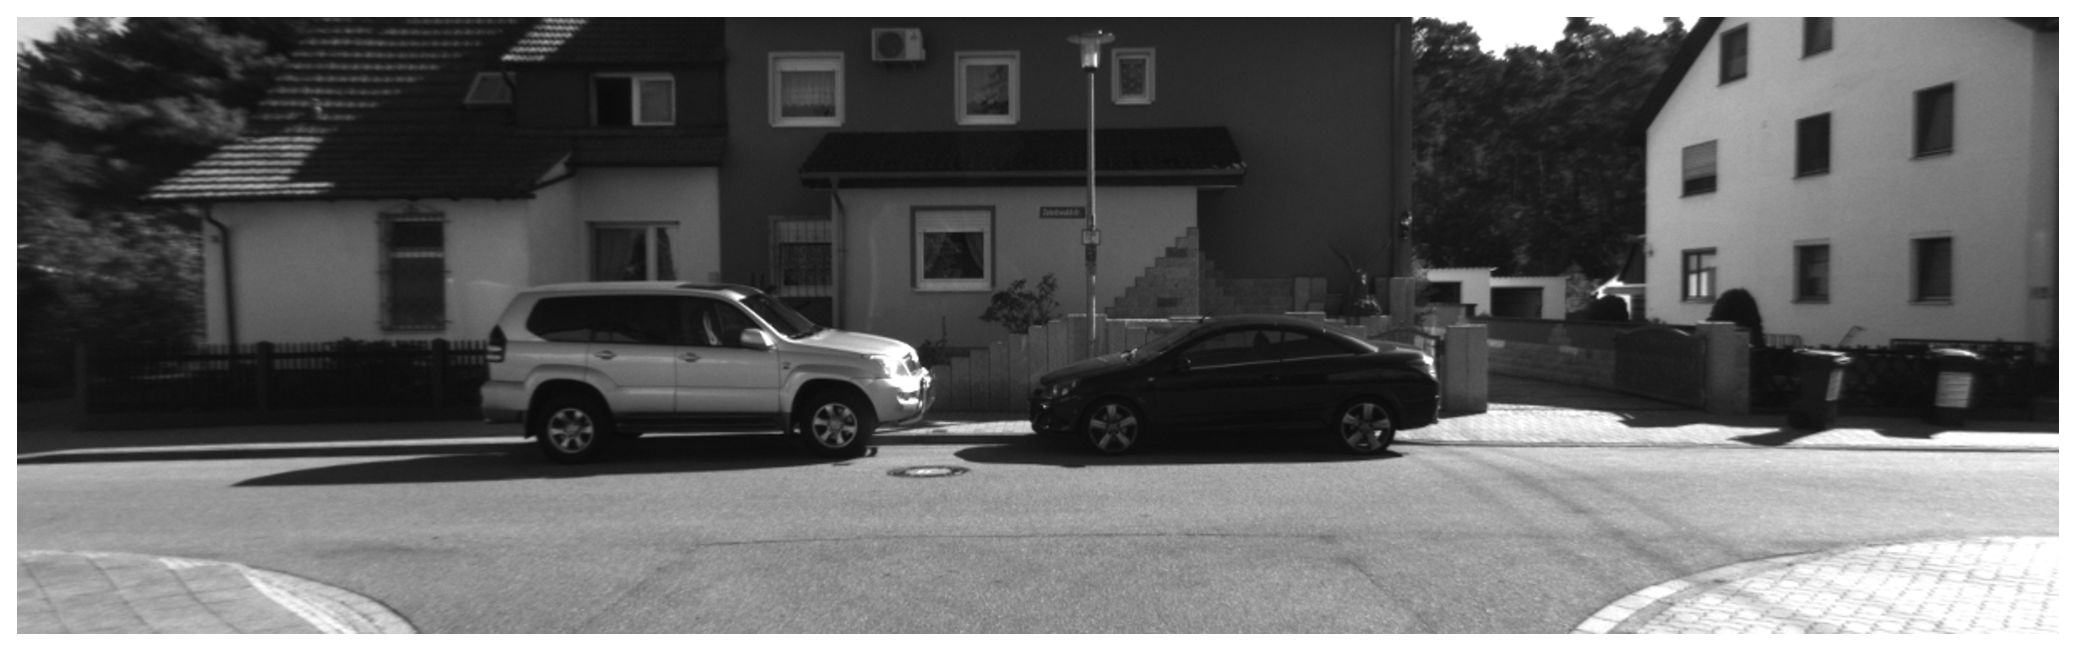
\includegraphics[scale=0.21]{000005L}}%
\subcaptionbox{Right image}
[.5\linewidth]{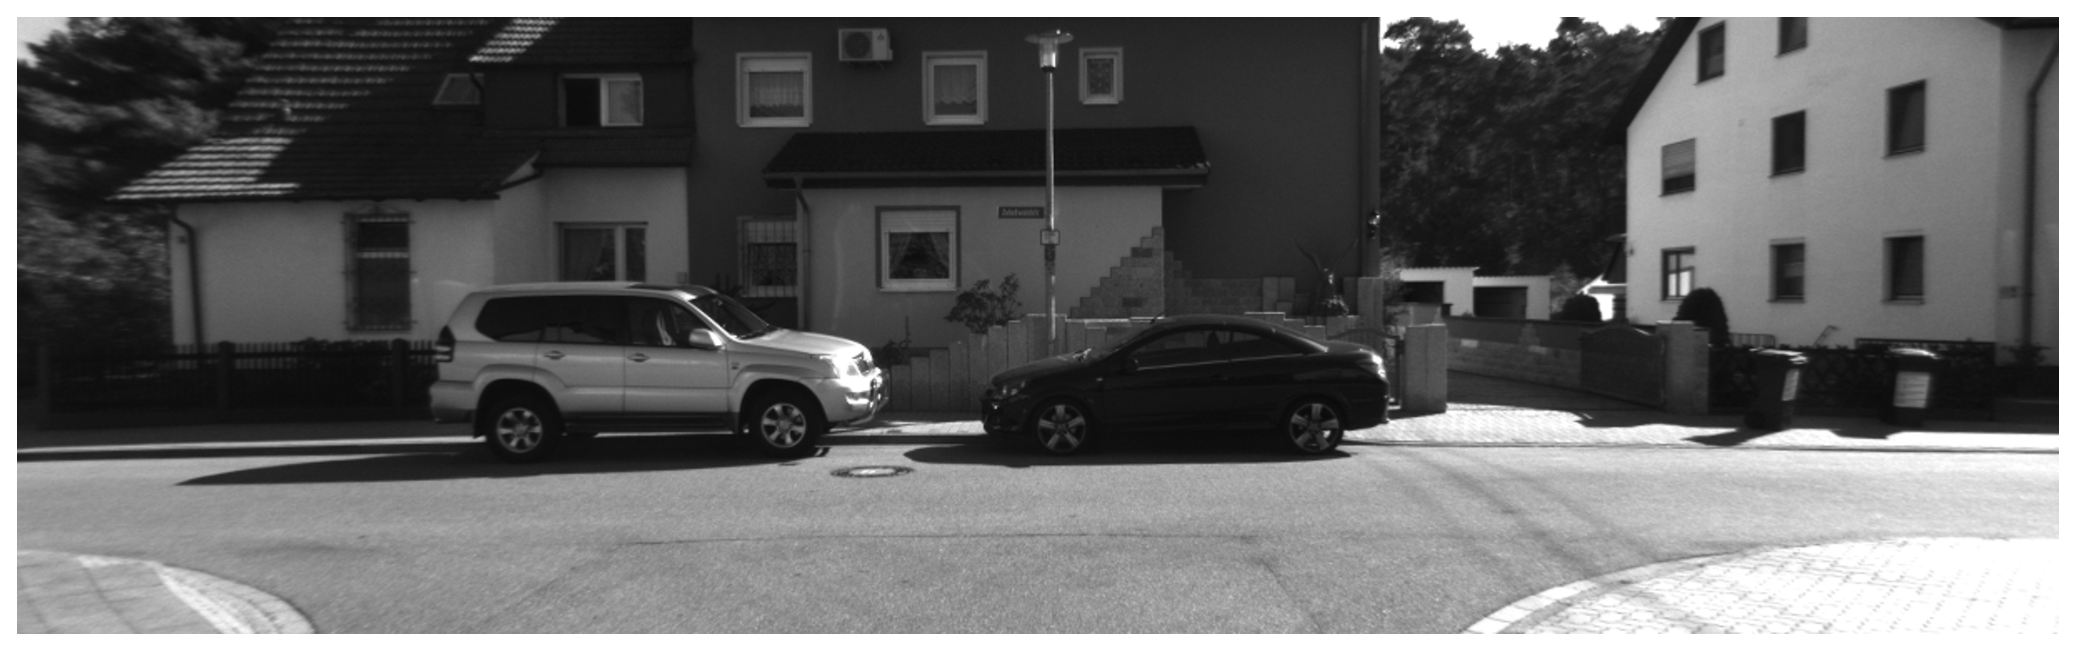
\includegraphics[scale=0.21]{000005R}}%
\caption{Sample stereo image from the Kitti dataset}
\label{fig:img5}
\end{figure}
\begin{figure}[H]
\centering
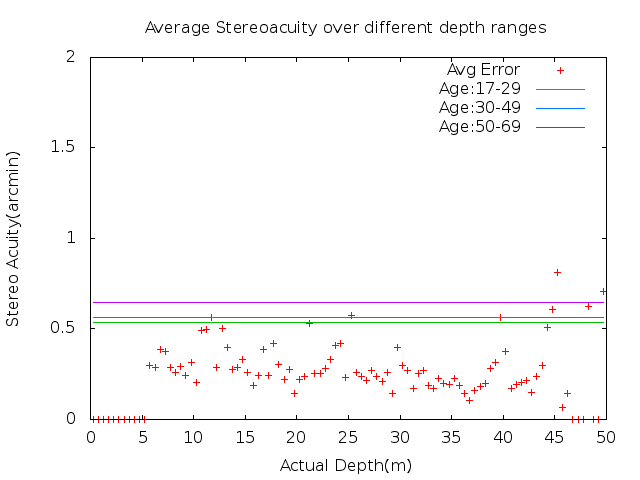
\includegraphics[scale=0.95]{sgbmimg5pix3msk}
\caption{Average disparity error over distance by SGBM for Figure \protect\ref{fig:img5}}
\label{fig:imgmsk5}
\end{figure} 
\begin{figure}[H]
\centering
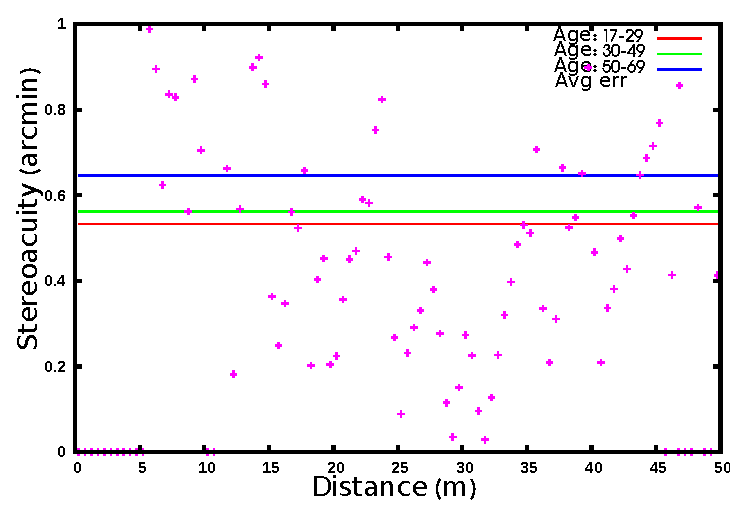
\includegraphics[scale=0.95]{adcimg5pix3msk}
\caption{Average disparity error over distance by ADCensusB for Figure \protect\ref{fig:img5}}
\label{fig:imgfull5}
\end{figure}

\noindent
The corresponding mask, Figure \ref{fig:msk}; masked ground truth, Figure \ref{fig:gtmsk}; and
the masked disparity images generated by SGBM and ADCensusB, Figures \ref{fig:5mdispsgb} and \ref{fig:5mdispadc} 
are shown below.

\begin{figure}[H]
\centering

\includegraphics[width=\linewidth, scale=0.48]{5msk}
\caption{The mask of depth edges and their surrounding regions for Figure \protect\ref{fig:img5}}
\label{fig:msk}
\end{figure} 
\begin{figure}[H]
\centering
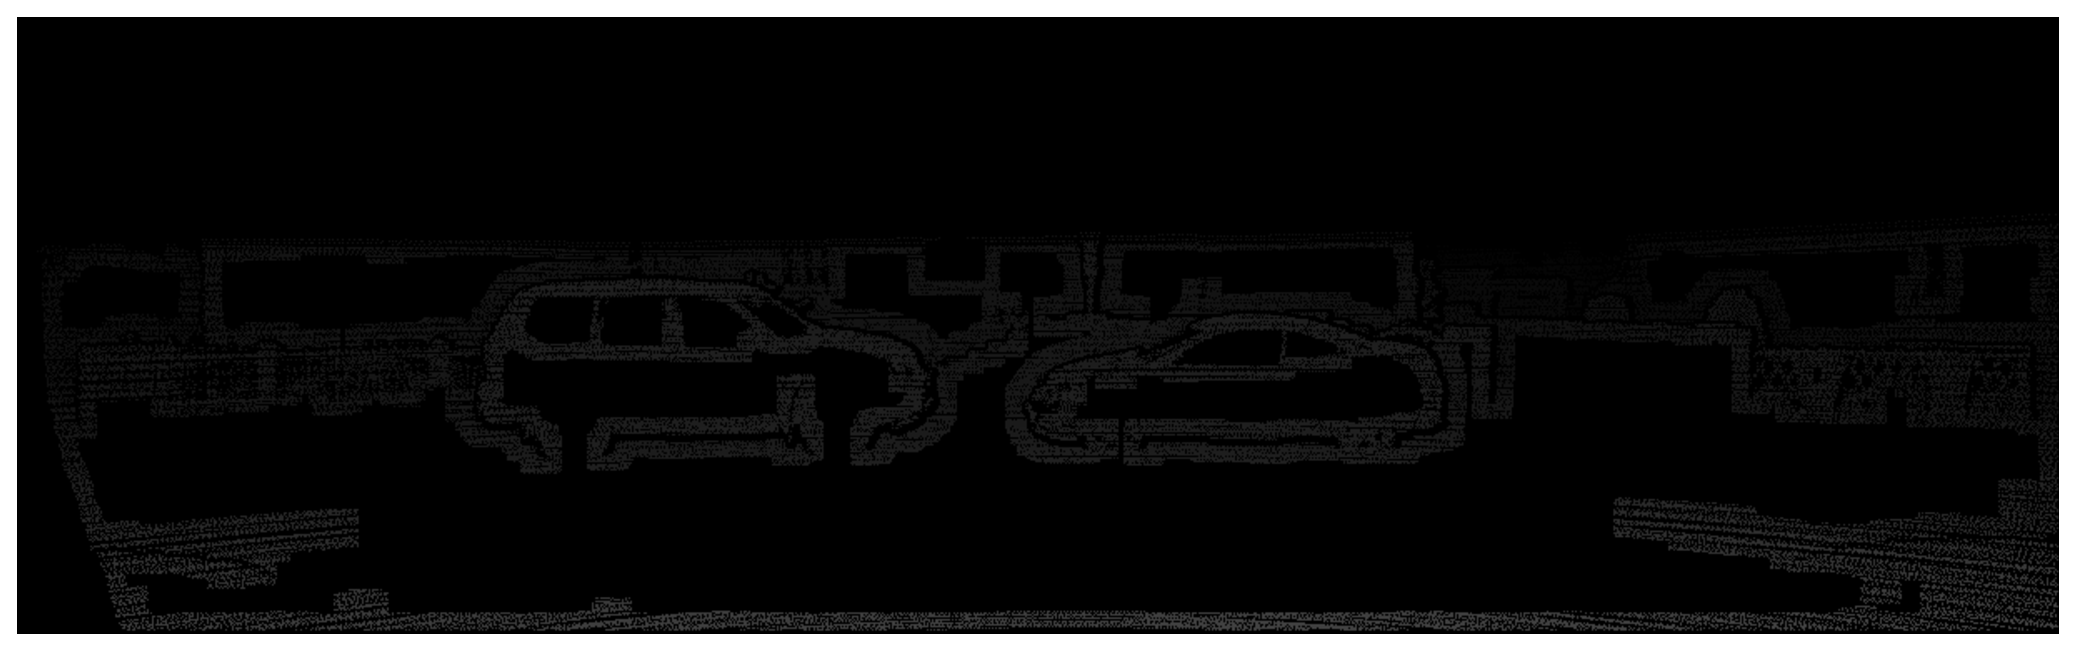
\includegraphics[width=\linewidth, scale=0.48]{5gt}
\caption{Masked ground truth for Figure \protect\ref{fig:img5}}
\label{fig:gtmsk}
\end{figure} 
\begin{figure}[H]
\centering

\includegraphics[width=\linewidth, scale=0.48]{5mdispsgb}
\caption{Masked disparity by SGBM for Figure \protect\ref{fig:img5}}
\label{fig:5mdispsgb}
\end{figure} 
\begin{figure}[H]
\centering

\includegraphics[width=\linewidth,scale=0.48]{5mdispadc}
\caption{Masked disparity by ADCensusB for Figure \protect\ref{fig:img5}}
\label{fig:5mdispadc}
\end{figure} 

\noindent
Figures \ref{fig:mskmapsgbm1000} and \ref{fig:mskmapadc1000} show the average results over all the disparity images for both SGBM and ADCensusB, respectively.

\begin{figure}[H]
\centering
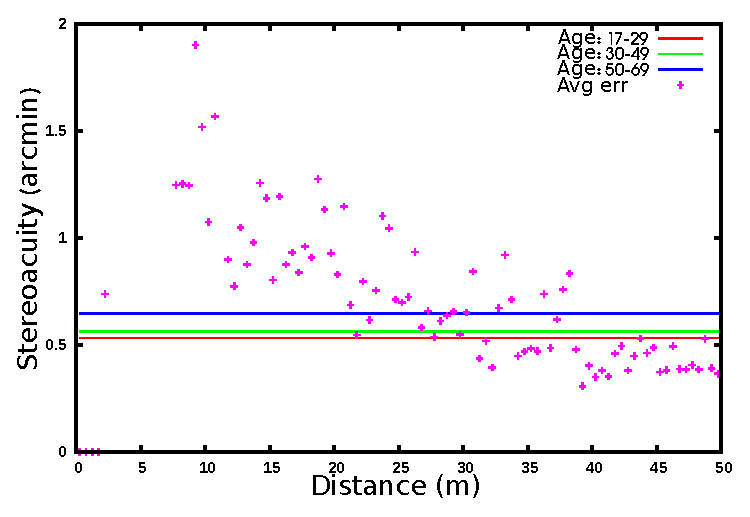
\includegraphics[scale=0.95]{sgbmmsk1000}
\caption{Average disparity error over all the images by SGBM}
\label{fig:mskmapsgbm1000}
\end{figure} 
\begin{figure}[H]
\centering
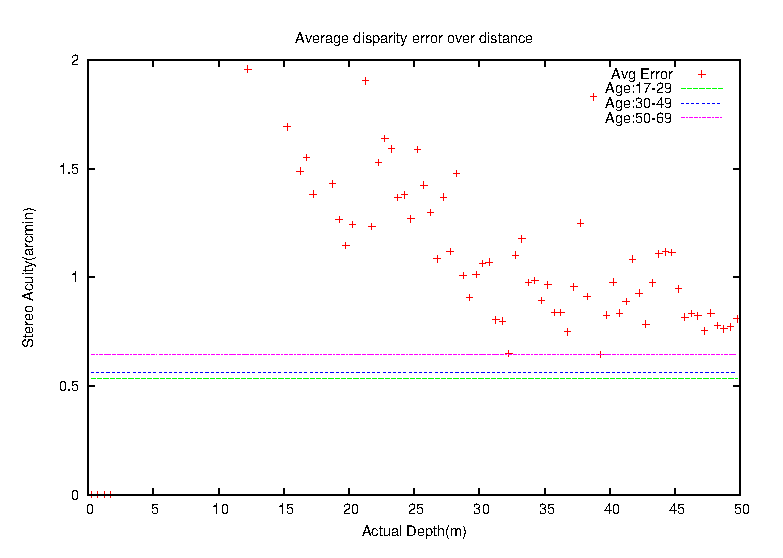
\includegraphics[scale=0.95]{adcenmsk1000}
\caption{Average disparity error over all the images by ADCensusB}
\label{fig:mskmapadc1000}
\end{figure} 

As can be seen, the average results displayed in the previous plots contain sparse points and 
do not demonstrate any consistent pattern. When we investigated the cause of this large variation, we found that in
the results of both algorithms, there are some disparity values which differ from the ground truth 
by a considerable amount and yet have not been invalidated by the
algorithm. We assume that these types of outliers can be easily removed from the set by applying a post processing filter, or 
they will be eventually culled out by the 3D renderer in the AR system. Based on this assumption, we fliter them out in our evaluation.
%Therefore, we have added another filtering condition to our evaluation module is similar to the approach employed by the
%Kiiti and Middlebury stereo evaluation. 
In order to filter out the disparity values which largely differ from the ground truth disparity, we have integrated another 
step in our evaluation process. This step is similar to the strategy used in the Kitti and Middlebury evaluation models.
In this step, the estimated disparity error is initially compared to a more generally defined threshold, for instance a threshold of 3 pixels.
This comparison allows only for those values of disparity with an error less than or equal to the specified threshold to 
move on to the next steps of the evaluation. It should be noted in our design, the specified threshold is defined as a run-time variable. \newline
The additional filtering had a significant impact on the evaluation results. In fact, a consistent pattern was observed in the final plots after filtering out the
outliers with large differences. The results are displayed in
figures \ref{fig:mskmapsgbm3} and \ref{fig:mskmapadc3}.

\begin{figure}[H]
\centering
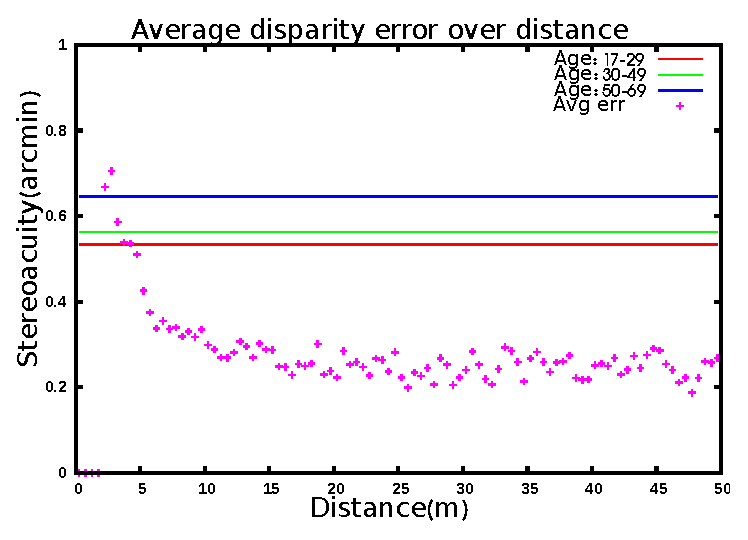
\includegraphics[scale=0.95]{sgbmmsk3}
\caption{Average disparity error over all the images by SGBM after filtering large outliers}
\label{fig:mskmapsgbm3}
\end{figure} 
\begin{figure}[H]
\centering
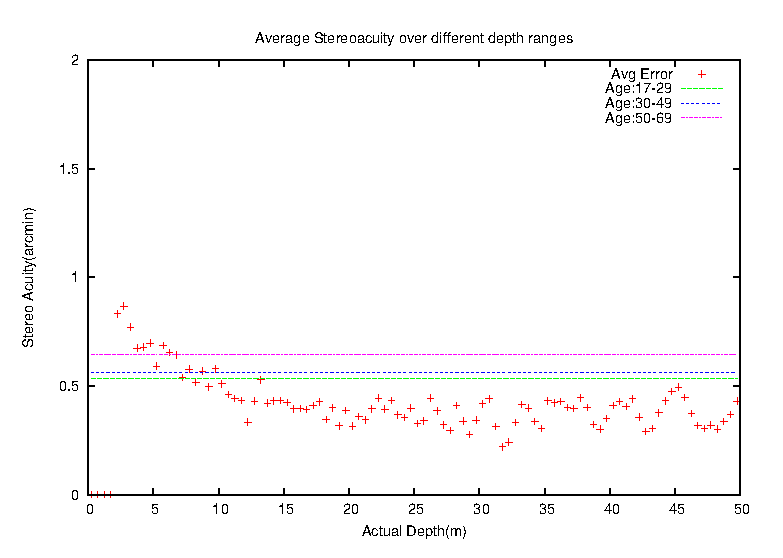
\includegraphics[scale=0.95]{adcenmsk3}
\caption{Average disparity error over all the images by ADCensusB after filtering large outliers}
\label{fig:mskmapadc3}
\end{figure} 

In these plots, a cross point below a stereoacuity threshold (straight lines) implies that the average error in the disparity values estimated 
by the stereo matching 
algorithm is imperceptible to the human visual system. However, a value higher than the threshold indicates that
the error cannot be ignored by the human visual system and should be resolved to achieve a better alignment between the virtual and the 
real world in the AR application of interest. Moreover, most of the errors
fall below the standard stereoacuity value corresponding to older ages; indicating that they are not perceptible to the visual system of the people at these 
particular ages.

The zero values in the plots imply that either there is no object within the corresponding range or the disparity value estimated by the algorithm
is equal to the ground truth disparity; however, since the average of the results has been taken over all the images, it is more likely that 
the zero values indicate that no object was found within the particular range.

As can be seen in the results, SGBM performs better in finding more accurate corresponding matches 
compared to ADCensusB, as most of the error points fall below the standard stereoacuity lines. Moreover, the plots show that in both methods 
the significant amount of error
corresponds to the near field objects, within the first 5 meters. This range of the depth field can be considerably important in some applications,
such as the ones involving certain manipulative tasks.

\subsection{Depth Edges and Occlusion}
In order to examine the effect of evaluating certain regions of the disparity image instead of the whole image, 
we estimated the average error both for the masked areas and the whole disparity map. 
Results of SGBM are shown in Figures \ref{fig:sgbmmsk3} and \ref{fig:sgbmfull3}.

\begin{figure}[H]
\centering
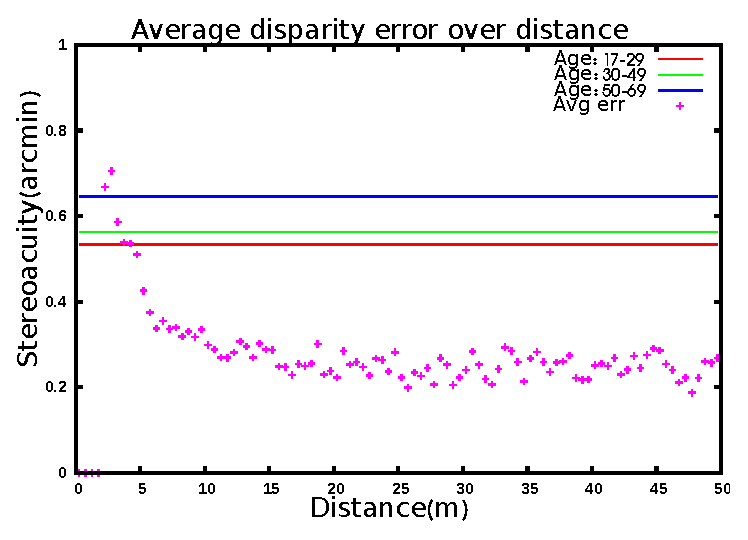
\includegraphics[scale=0.95]{sgbmmsk3}
\caption{Average disparity error over masked areas by SGBM}
\label{fig:sgbmmsk3}
\end{figure} 
\begin{figure}[H]
\centering
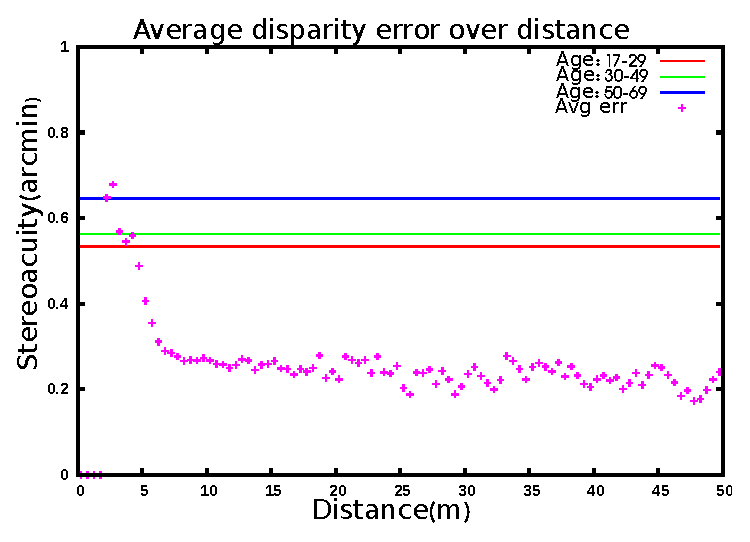
\includegraphics[scale=0.95]{sgbmfull3}
\caption{Average disparity error over the whole image by SGBM}
\label{fig:sgbmfull3}
\end{figure} 

The plots show that the average error over the masked regions, that is near the depth edges, is very similar to the results over the whole image. 
This may imply that there is no additional benefit in the inspection of these regions. 
However, this might be merely an indication of the performance of the selected algorithms and can be better analyzed by evaluating more algorithms 
within our model.
In either case, we hypothesize that, due to the importance of occlusion and areas near depth discontinuities to the HVS \cite{sze11},
it is reasonable to focus more on the depth edges and their surroundings when designing or employing a stereo matching technique for an AR application.

\subsection{Average Outliers}
In this experiment the average outliers were measured for both algorithms. 
The values for both validity criteria mentioned in chapter \ref{chap:System}, valid pixels in the ground truth and generated disparity, 
are presented in Tables \ref{tab:outlmsk} and \ref{tab:outlfull} for each age group. For simplicity, we have labelled the valid pixels
in the ground truth and the generated disparity with \textbf{valid\_gtDisp} and \textbf{valid\_genDisp}, respectively.
Figure \ref{fig:outlbar} presents a comparison between all the results for one of these validity criteria, when the ground truth disparity is valid. \newline

%{\footnotesize
\begin{minipage}{\linewidth}
\begin{center}
\captionof{table}{Average outliers for the masked regions}
\label{tab:outlmsk}
\begin{tabular}{ |c|c|c|c| }
\hline
\multicolumn{2}{|c}{} & \multicolumn{2}{|c|}{Avg\_Outliers} \\
\hline
Algorithm & Age & valid\_gtDisp & valid\_genDisp \\ \hline
\multirow{4}{*}{SGBM} & 17-29 & 0.12 & 0.16 \\
& 30-49 & 0.11 & 0.15 \\
& 50-69 & 0.09 & 0.12 \\
& 70-83 & 0.0012 & 0.0016 \\ \hline
\multirow{4}{*}{ADCensusB} & 17-29 & 0.23 & 0.32 \\
& 30-49 & 0.22 & 0.31 \\
& 50-69 & 0.18 & 0.27 \\
& 70-83 & 0.002 & 0.003 \\ \hline
\end{tabular}
\end{center}
\end{minipage} \newline \newline
%}

\begin{minipage}{\linewidth}
\begin{center}
\captionof{table}{Average outliers for the whole image}
\label{tab:outlfull}
\begin{tabular}{ |c|c|c|c| }
\hline
\multicolumn{2}{|c}{} & \multicolumn{2}{|c|}{Avg\_Outliers} \\
\hline
Algorithm & Age & valid\_gtDisp & valid\_genDisp \\ \hline
\multirow{4}{*}{SGBM} & 17-29 & 0.11 & 0.14 \\
& 30-49 & 0.10 & 0.12 \\
& 50-69 & 0.08 & 0.09 \\
& 70-83 & 0.005 & 0.007 \\ \hline
\multirow{4}{*}{ADCensusB} & 17-29 & 0.27 & 0.39 \\
& 30-49 & 0.26 & 0.37 \\
& 50-69 & 0.22 & 0.32 \\
& 70-83 & 0.002 & 0.003 \\ \hline
\end{tabular}
\end{center}
\end{minipage} \newline \newline

Results in Figure \ref{fig:outlbar} show that in both cases, the masked regions and the whole image, SGBM has less outliers than ADCensusB, indicating that
SGBM generates a more accurate disparity map as perceived by the human visual system.
Another observation from Figure \ref{fig:outlbar} is that in SGBM, the average outliers over the masked regions are more than the outliers over the whole image, whereas in ADCensusB the
opposite behavior is observed. This implies that SGBM generates less accurate results
near the depth discontinuities and occluded regions compared to the other areas in the image.
On the other hand, ADCensusB generates more accurate disparity values near the depth edges compared to the other regions in the image and 
tends to preserve the occluded regions. This indicates that, despite the better performance of SGBM over ADCensusB according to the
experimental results, it is important to consider this behavior to employ the stereo correspondence method
in the right application based on the requirement of the target system for the accuracy of the depth results in different regions; in other
words, it is reasonable to first investigate which regions in the image are more important in the context of the target application.
%whether the accuracy near the depth discontinuities and preserving the occlusion is more important than the
%other regions in the image or not.
For instance, ADCensusB performs better in an application where the areas
near the depth discontinuities and occlusion are more important than the rest of the image, such as image compositing for layering visual elements
on the scene, compared to application scenarios where obtaining an accurate, dense disparity map for all the regions in an image is essential, such as
constructing a 3D model of the scene or preparing a model for 3D printing.


\begin{figure}[H]
\centering
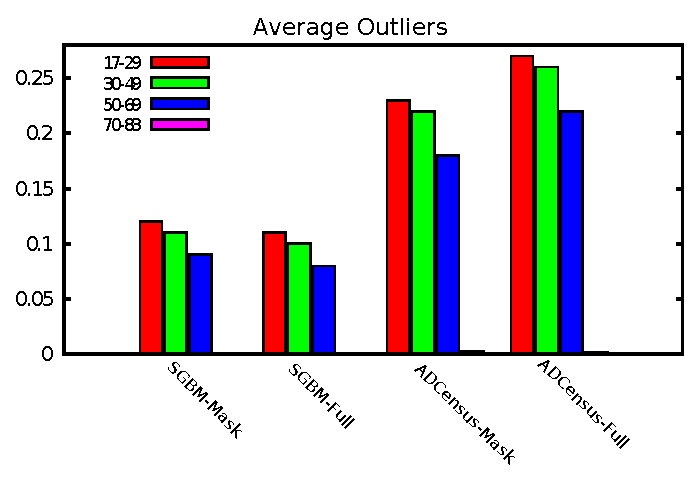
\includegraphics[scale=0.95]{outlchart}
\caption{Average outliers for SGBM and ADCensusB over the masked and the whole image; each bin color corresponds to different age groups with specific stereoacuity threshold}
\label{fig:outlbar}
\end{figure} 

%Furthermore, in SGBM the number of outliers over the masked regions are more than the outliers over the whole image, whereas in ADCensus the
%opposite behavior is observed; that is the number of outliers over the masked regions are less than 
%the whole image. This implies that ADCensus performs better in the areas of depth edges and their surroundings than other regions.
%Therefore, it is better to be employed in the applications where preserving the object boundaries and occluded areas
%is adequate and more important than the other regions in the image, such as image compositing for layering visual elements
%on the scene. However, this metric per se
%cannot be an indicator of the suitability of the solution for any target application and should be considered along with the other
%relevant metrics. 
We should note that the reason the number of outliers for the valid pixels in the generated disparity is more than the outliers for the valid pixels
in the ground truth is that in our implementation, the counter for the number of pixels in the ground truth image 
is incremented whenever a disparity pixel in the ground truth is labelled as valid, regardless of other conditions in the process; 
however, the counter for the number of pixels in the generated disparity
is only incremented whenever the disparity value is valid and the amount of disparity error is less than the specified pixel threshold in the evaluation process, thus resulting
in a smaller denominator of the fraction in the estimation of the average outliers for the criteria of valid pixels in the generated disparity map and, therefore, a larger 
average value in the end.

\subsection{Average Disparity Error}
The average disparity error has also been estimated in the evaluation process for both pixel validity criteria. However, the resulting values
were similar for both cases and, therefore, only one value is reported in the following table for this metric. \newline

\begin{minipage}{\linewidth}
\begin{center}
\captionof{table}{Average disparity error}
\label{tab:avgerr}
\begin{tabular}{ |c|c|c| }
\hline
Algorithm & Region & Avg\_DispErr \\ \hline
\multirow{2}{*}{SGBM} & Full & 6.58 \\ \cline{2-3}
& Masked & 7.81 \\ \hline
\multirow{2}{*}{ADCensusB} & Full & 4.49 \\ \cline{2-3}
& Masked & 4.74 \\ \hline
\end{tabular}
\end{center}
\end{minipage} \newline \newline

As can be seen, ADCensusB results in less average disparity error than SGBM. This difference is likely caused by the various refinement steps
implemented in the ADCensusB algorithm which do not exist in SGBM.
As a result, despite the larger number of outliers in ADCensusB than SGBM as measured in the previous experiments,
ADCensusB attempts to decrease the difference between the resulting disparity value and the ground truth disparity, thus generating smoother disparity patches
within different regions of the images.

\subsection{Real-time Execution}
In another experiment, we estimated the average execution time for both algorithms. Results show that the average execution time over all the images 
for SGBM and ADCensusB are $0.54$ and $272.82$ seconds, respectively.
Considering the requirements of having an interactive real-time AR system \cite{hertz00}, the processing time of each frame should not be more than 0.06-0.08 seconds.
Although the current implementation of SGBM could be used when the real world scene remains stable for approximately one second, it can be safely concluded that
none of these algorithms meet the requirements of a real-time interactive AR system.
This suggests that GPU-based solutions are more suitable to achieve the processing speed required for the real-time 
interactive applications of AR. In \cite{mei11}, it is stated that the GPU implementation of ADCensus brings $140\times$ speedup in the processing speed.

\subsection{Effect of Refinement}
In this experiment, we studied the effect of the post processing steps, also referred to as the \textit{refinement steps}, 
in the stereo algorithms on the accuracy of the results in our evaluation criteria. 

Refinement is usually the last step in a stereo correspondence algorithm because it attempts to decrease the 
number of wrong matches or the error after the disparity results have been found \cite{sch02}. Therefore, this step must be applied after the outliers, that is the wrong pixel matches, 
have been detected in the results.
The detection of the outliers occurs through a check known as left-right consistency check in a stereo matching algorithm. In this check, the disparity map for both
the left and right image is first calculated. Then, if a pixel in the left image, based on its disparity value, corresponds to a pixel in the right image
that does not map back to it, it will be labeled as an outlier \cite{sch02}. This description can be formulated as follows:

\begin{align}
D_{L}(p) \neq D_{R}(p-(D_{L},0))
\end{align}
\noindent
Where $D_{L}(p)$ is the disparity function for the left image and $D_{R}$ is the disparity function for the right image. \newline
For simplicity, we will refer
to this check as L-R check in this report.
In our implementation of ADCensus, we have the L-R check and its subsequent refinement steps triggered with a flag.
Therefore, when the flag is not set, neither the check nor the refining steps are triggered in the algorithm.
To investigate the effect of the refinement on the final results, we used 
ADcensus in this experiment with the L-R flag set to zero, generating the disparity results for the image pairs, and evaluating the results.
The results for both cases, not refined and refined, over the masked regions and the whole image are shown in Figures \ref{fig:adcMLRnoLR} and \ref{fig:adcFLRnoLR}, respectively.

\begin{figure}[H]
\centering
\begin{subfigure}{\linewidth}
\centering
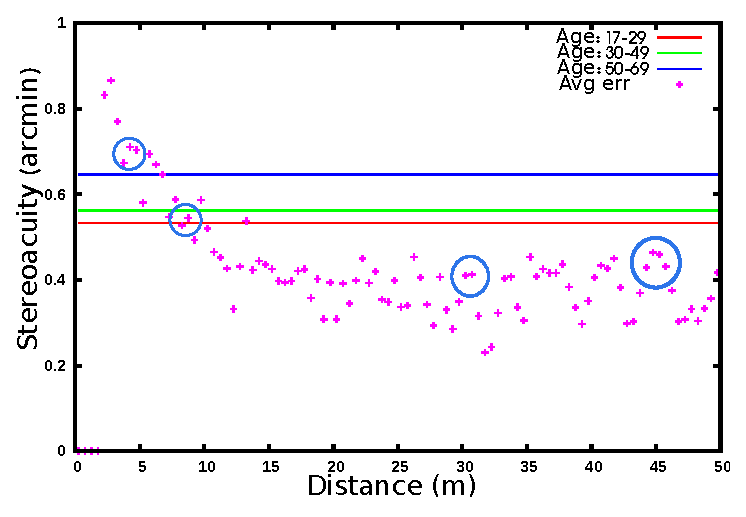
\includegraphics[scale=0.95]{adcenmsk3NoLRmrk}
\caption{No refinement on disparity results}
\label{fig:adcmnoLR}
\vspace{2mm}
\end{subfigure}\\
%\end{figure} 
\begin{subfigure}{\linewidth}
\centering
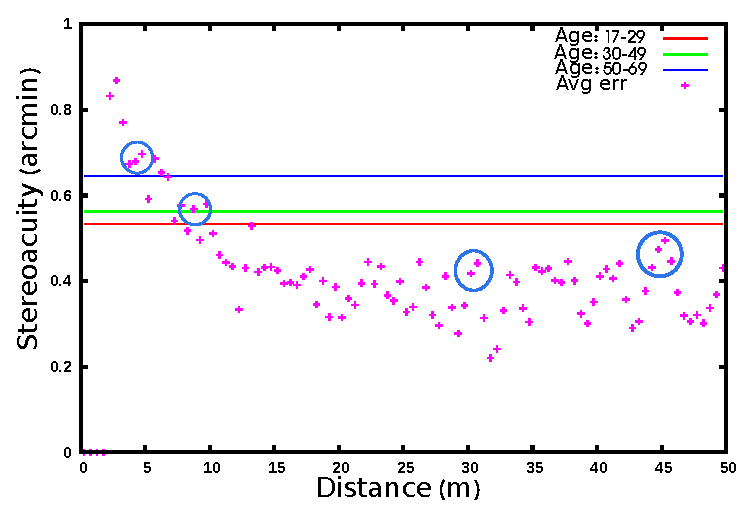
\includegraphics[scale=0.95]{adcenmsk3mrk}
\caption{Refinement on disparity results}
\label{fig:adcm3mrk}
\end{subfigure}
\caption{Average disparity error by ADCensusB for the masked images; Blue circles show some sample values that have slightly changed as a result of refinement}
\label{fig:adcMLRnoLR}
\end{figure} 

\begin{figure}[H]
\centering
\begin{subfigure}{\linewidth}
\centering
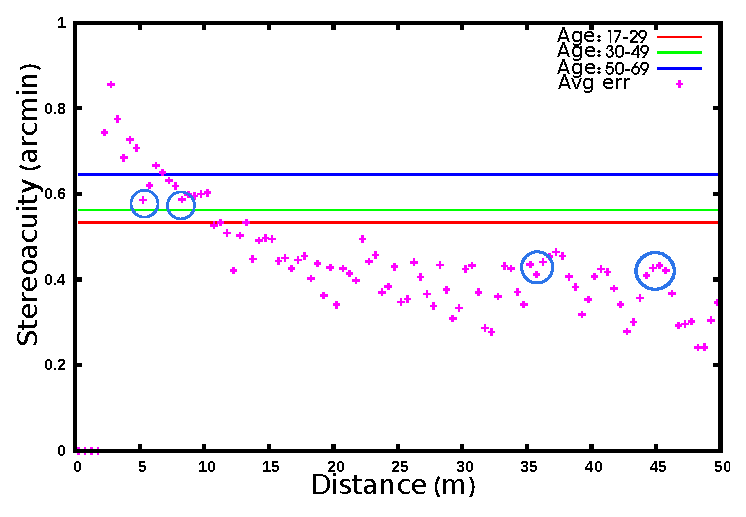
\includegraphics[scale=0.95]{adcenfull3NoLRmrk}
\caption{No refinement on disparity results}
\label{fig:adcfnoLR}
\vspace{2mm}
\end{subfigure} \\
%\end{figure} 
\begin{subfigure}{\linewidth}
\centering
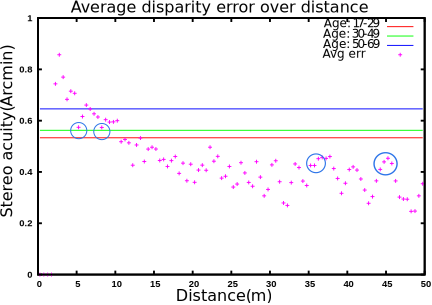
\includegraphics[scale=0.95]{adcenfull3mrk}
\caption{Refinement on disparity results}
\label{fig:adcf3mrk}
\end{subfigure}
\caption{Average disparity error by ADCensusB for the whole images; Blue circles show some sample values that have slightly changed as a result of refinement}
\label{fig:adcFLRnoLR}
\end{figure} 

As can be observed in the plots, the evaluation results in our specific criteria 
are not significantly different from the results of the algorithm when L-R check and refinement were triggered
and only a few average values have slightly changed. We have marked a few of these values with blue circles in Figures \ref{fig:adcMLRnoLR}, \ref{fig:adcFLRnoLR}. \newline
We also estimated the average execution time, the average disparity error, and the average outliers in this experiment. The results for 
the average error and outliers are shown in the tables below. \newline

\begin{minipage}{\linewidth}
\begin{center}
\captionof{table}{ADCensusB average disparity error - unrefined}
\label{tab:adcerrNref}
\begin{tabular}{|c|c|}
\hline
Region & Avg\_DispErr \\ \hline
Masked & 5.59 \\  \hline
Full & 5.29 \\ \hline
\end{tabular}
\end{center}
\end{minipage} \newline \newline

\begin{minipage}{\linewidth}
\begin{center}
\captionof{table}{ADCensusB average outliers - unrefined}
\label{tab:adcoutlNref}
\begin{tabular}{ |c|c|c|c| }
\hline
\multicolumn{2}{|c}{} & \multicolumn{2}{|c|}{Avg\_Outliers} \\
\hline
Region & Age &  valid\_gtDisp & valid\_genDisp \\ \hline
\multirow{4}{*}{Masked} & 17-29 & 0.23 & 0.33 \\
& 30-49 & 0.22 & 0.31 \\
& 50-69 & 0.18 & 0.27 \\
& 70-83 & 0.002 & 0.003 \\ \hline
\multirow{4}{*}{Full} & 17-29 & 0.27 & 0.39 \\
& 30-49 & 0.26 & 0.37 \\
& 50-69 & 0.23 & 0.32 \\
& 70-83 & 0.001 & 0.002 \\ \hline
\end{tabular}
\end{center}
\end{minipage} \newline \newline

Figure \ref{fig:outlnoref} shows a comparison between the average outliers by ADCensusB with the effect of refinement and without it for the masked and the whole images 
in one of the validity criteria, that is, when the ground truth disparity is valid. As can be seen, no significant decrease is obtained in the number of outliers.

\begin{figure}[H]
\centering
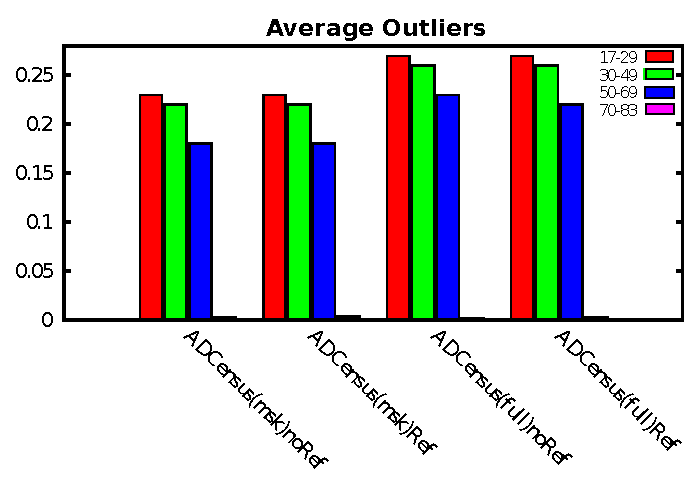
\includegraphics[scale=0.95]{adcrefNoref}
\caption{Average disparity error by ADCensusB in refined and unrefined cases for both masked and whole images; Different colored bins correspond to different age groups
with specific stereoacuity thresholds}
\label{fig:outlnoref}
\end{figure} 

The average execution time was approximately $147.84$ seconds which is nearly half the running time of the algorithm with the L-R check and refinements 
triggered, Table \ref{tab:timerefNoref}. 
Comparing these results to the ones presented in Tables \ref{tab:outlmsk}, \ref{tab:outlfull}, and \ref{tab:avgerr} a slight decrease in the amount of errors and 
nearly no change in the number of outliers is observed.
Analyzing the results in this experiment, we can conclude that despite the considerable rise in the execution time of the algorithm, no significant
improvement in accuracy is achieved in our evaluation criteria through refinement of the disparity results; therefore, the execution of ADCensusB without any L-R check and
refinement step is more beneficial to an AR application in outdoor environments, since it requires less processing time.\newline

\begin{minipage}{\linewidth}
\begin{center}
\captionof{table}{ADCensusB average execution time - refined and unrefined}
\label{tab:timerefNoref}
\begin{tabular}{|c|c|}
\hline
ADCensusB & Avg\_ExecTime (secs) \\ \hline
refined & 272.82 \\  \hline
unrefined & 147.84 \\ \hline
\end{tabular}
\end{center}
\end{minipage} \newline

\subsection{Discretization Degree of Disparity Values}
According to different studies \cite{dras96, kru10,azuma01}, some other factors such as issues associated with the environment, display device, and capturing device
can also affect the perception of depth in the visual system. As a result, the ability to detect the difference in depth and accurately estimate the
depth of different points, in practice,
do not merely depend on the implemented discretization level of the disparity values in the stereo correspondence algorithm.
In order to investigate the validity of this statement, we conducted the following experiment. In this experiment we defined some stereoacuity thresholds. 
In order to find the minimum threshold to start with, we attempted to find the 
minimum disparity change in the ground truth disparity images. To this end, we move along horizontal scanlines in each image and 
compute the difference between the values of consecutive pixels, which is, in fact, an indicator of the detectable threshold of the changes in depth between
different pixels, Figure \ref{fig:scanline}. 

\begin{figure}[H]
\centering
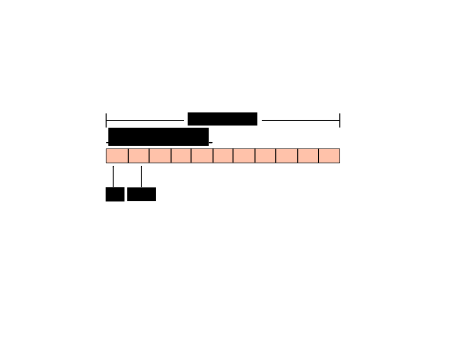
\includegraphics{scanline}
\caption{The scanline pixels difference process}
\label{fig:scanline}
\end{figure} 

After finding the minimum value in each image, a global minimum is sought between all the computed values from different images.
The value we found for a group of twelve images selected from our dataset with the size of $1242\times375$ and the focal length of $721$ 
millimeters was $0.0022$ arcmins.
After finding this minimum and defining our thresholds, we apply a nearly similar operation on the disparity results of the same group of images 
from each of the sample algorithms.
In this process, while moving through each image, for those pixels whose generated disparity is close to the ground truth disparity, 
within a specific pixel threshold, 
we estimate their depth difference from their following pixel
in the ground truth and compare the value to each of the specified thresholds; if this value is less than a threshold, then we check to see whether
the stereo algorithm has also detected different values for the corresponding pixels. 
In case of detection, we increment a counter corresponding to each threshold that indicates the number of detected pixels.
This process is repeated for different images and, finally, the average of detected pixels is estimated for each specified threshold.

\begin{alltt}
\textbf{ADP}; START
      define StAc\_thresh;
      for all images; do
         for all pixels p in the image:
            if (\( |disp\sb{gt}-disp\sb{gen}|<pix\_thresh\))
               \(pix\_count += 1\);
               \(dispDiff = |disp\sb{gen\sb{p}}-disp\sb{gen\sb{p+1}}|\);
               \(depth\sb{gt\sb{p}} = \frac{focal\_length \times baseline}{disp\sb{gt\sb{p}}}\);
               \(depth\sb{gt\sb{p+1}} = \frac{focal\_length \times baseline}{disp\sb{gt\sb{p+1}}}\);
               \(depthDiff = |depth\sb{gt\sb{p}}-depth\sb{gt\sb{p+1}}|\);
               \(stAc\_detected = \frac{pupil\_distance*depthDiff}{depth\sb{gt\sb{p}}\sp{2}}\);
               for each threshold \textit{thr} in StAc\_thresh:
                  if (\(stAc\_detected<thr\))
                     if (\(dispDiff>0\))
                        \(detected[thr]++\);
                     end if
                  end if
               end for
            end if
         end for
         for each threshold \textit{thr} in StAc\_thresh:
            \(Avg\_detected[thr] = detected[thr]/pix\_count\);
            Append(Avg\_pixFile, \(Avg\_detected[thr]\));
         end for
      end for
      /**Concatenate the files for all images into one **/
      for each Avg\_pixFile:
         Concat(AllimgFile,Avg\_pixFile);
      end for
      /**Getting the average over all images for each threshold**/
      Calc\_Average(AllimgFile, OutAvgFile);
      plot(OutAvgFile);
\textbf{ADP}; END
\end{alltt}
The results for both algorithms are shown in Figure \ref{fig:algthresh}.
As can be seen in these plots, for both algorithms, the average detected pixels with detectable change in depth values 
starts to converge at the value of approximately $0.4$ arcmins.
We also observe that for the values below this threshold the average detected pixels are very small and for some values, 
such as the minimum detectable threshold in ground truth,
both algorithms are not capable of detecting any change in depth values. 
This implies that, regardless of the accuracy resolution of the algorithms, which is $1/8$th of a pixel for SGBM and $1/16$th of a pixel for ADCensusB, approximately equal to
$0.6$ arcmins and $0.3$ arcmins, respectively, for Kitti images based on the camera parameters and the geometrical relation presented in Figure \ref{fig:camResolution} and 
Equation \ref{eq:algResolution}, some changes in 
depth in the real world cannot be still detected by the algorithm. This effect might be due to the constraints of the sensor, that is, the errors associated with the capturing 
device and its resolution, or the environmental noise. 

\begin{figure}[H]
\centering
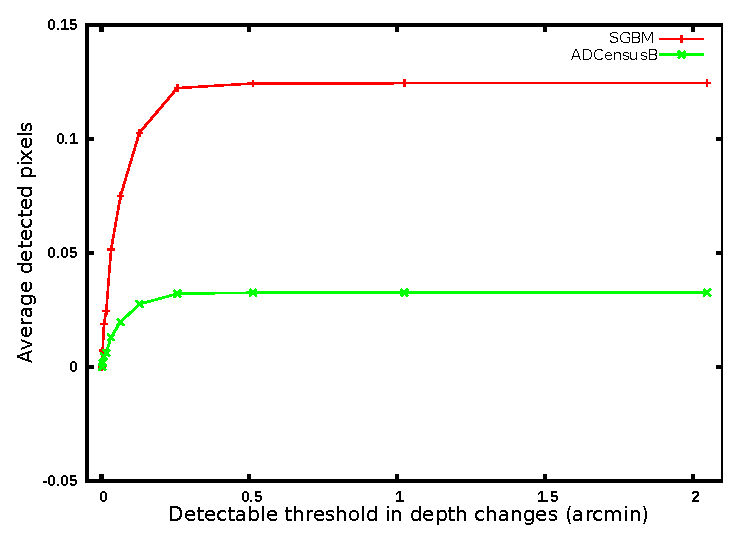
\includegraphics{algthreshBoth}
\caption{Average detected pixels by SGBM and ADCensusB for specific stereoacuity thresholds marked on each curve}
\label{fig:algthresh}
\end{figure} 
\begin{figure}[H]
\centering

\includegraphics{camRes}
\caption{Resolution of image in angular disparity}
\label{fig:camResolution}
\end{figure}

\noindent
In Figure \ref{fig:camResolution}, $w$ is the image width and $f$ is the focal length of the capturing device.

\begin{align}
\label{eq:algResolution}
\theta = \arctan(\frac{pixel\_resolution}{focal\_length})
\end{align}

For the image size of $1242\times375$ pixels and focal length of $721$ millimeters, and based on the resolution of SGBM and ADCensusB in the estimation of the disparity values, 
the minimum and maximum detectable disparity, that is, at the center and at the boundary of the image, respectively, 
in terms of effective stereoacuity are as follows:

\begin{align}
\label{eq:algsgbmresolv} 
&\begin{aligned}
SGBM: \theta_{max} &= \arctan (\frac{\frac{1}{8}}{721}) \\
&= 0.00993 \text{ degrees} \times 60 \frac{arcmins}{degrees} = 0.596 \text{ arcmins}
\end{aligned}\\[2ex]
&\begin{aligned}
SGBM: \theta_{min} &= \arctan (\frac{\frac{1}{8}\times(\frac{1242}{2})}{721}) - \arctan (\frac{\frac{1}{8}\times(\frac{1242}{2}-1)}{721}) \\
&= 0.00982 \text{ degrees} \times 60 \frac{arcmins}{degrees} = 0.589 \text{ arcmins}
\end{aligned}\\[2ex]
&\begin{aligned}
ADCensusB: \theta_{max} &= \arctan (\frac{\frac{1}{16}}{721}) \\
&= 0.00496 \text{ degrees} \times 60 \frac{arcmins}{degrees}= 0.298 \text{ arcmins} 
\label{eq:adcenresolv}
\end{aligned}\\[2ex]
&\begin{aligned}
ADCensusB: \theta_{min} &= \arctan (\frac{\frac{1}{16}\times(\frac{1242}{2})}{721}) - \arctan (\frac{\frac{1}{16}\times(\frac{1242}{2}-1)}{721}) \\
&= 0.00495 \text{ degrees} \times 60 \frac{arcmins}{degrees}= 0.297 \text{ arcmins}
\end{aligned}
\end{align} \newline
\noindent
However, as can be seen, the minimum and maximum angular resolution in the image are not considerably different.

As a result of this experiment, we can conclude that in order to achieve 
more accurate depth values in the stereo algorithms and better detectability of their changes, 
in areas of depth discontinuities, that is, to obtain a lower 
threshold of depth changes
closer to the actual resolution of the implemented algorithm, using higher resolution devices and considering their robustness to noise are also essential.
However, the experimental results presented earlier in this chapter
show that despite various types of error relevant to the capturing device, environmental noise, and the accuracy of the stereo correspondence algorithm
in the estimation of disparity values, the effect of such error on the results, depending on the distance of the object from the observer, 
will not be perceptible in the HVS for outdoor AR applications.

\section{Overview}
Table \ref{tab:compare} shows an overview of the difference between our proposed evaluation approach and the other evaluation models, Middlebury
and Kitti, in terms of the estimated evaluation metrics. \newline
It should be noted that although the average error and the average outliers exist in the other evaluation schemes as well, the major
difference which makes our evaluation more appropriate than the other schemes for practical applications of AR,
is the approach employed during the design of the metrics and the analysis of the results in the evaluation process. In fact, integrating the 
important factors related to the human visual system and its
perception of depth in the design of the metrics and the insights they provide make the evaluation model more relevant and applicable to outdoor AR systems. \newline

%{\footnotesize
\begin{minipage}{\linewidth}
\begin{center}
\captionof{table}{Comparison of different evaluation schemes}
\label{tab:compare}
\begin{tabular}{ |c|c|c|c| }
\hline
\textbf{Metrics} & \multicolumn{3}{|c|}{\textbf{Evaluation Models}}  \\ \hline
& \textit{Middlebury} & \textit{Kitti} & \textit{Comprehensive\_Evaluation} \\ \hline
\textit{Avg\_StAc} & \ding{55} & \ding{55} & \ding{51} \\ \hline
\textit{Avg\_Outliers} & \ding{51} & \ding{51} & \ding{51} \\ \hline
\textit{Avg\_DispErr} & \ding{51} & \ding{51} & \ding{51} \\ \hline
\textit{Avg\_ExecTime} & \ding{55} & \ding{55} & \ding{51} \\ \hline
\end{tabular}
\end{center}
\end{minipage} \newline
%}

\section{Hypotheses Validation}
Next, we will review our hypotheses mentioned earlier in this chapter and discuss their validity in light of our experiments and their results.

\begin{itemize}
\item \textbf{Hypothesis 1}: \emph{Our model is more suitable than other approaches to evaluate and demonstrate
the performance of the stereo matching algorithm in the framework of 
outdoor augmented reality applications.} 

As can be seen in the results of the experiments, our system employs a systematic approach for the measurement and demonstration of different 
evaluation metrics in the framework of an outdoor augmented reality application. 
In our system, the disparity error, which is the most important metric for the accuracy of the disparity results, 
is converted to a certain measurement, stereoacuity, that is relevant and applicable to the human visual
system and its perception of depth. We evaluated two stereo matching methods in our system and analyzed their performance in terms of
the accuracy of the depth map for an outdoor AR application. Due to the application-oriented design of the system, we could comment on the suitability of each method
for an AR application in outdoor environments. As a result, we can argue that our evaluation model is more appropriate for the evaluation of the solutions 
in an outdoor AR system than the conventional evaluation systems.

\item \textbf{Hypothesis 2:} \emph{Observing, evaluating, and consequently 
refining the areas near the depth edges in an image are more important in an AR application.}

The results of our experiments on two sample stereo matching solutions showed no significant difference between the evaluation metrics corresponding to the whole image and
the regions of the depth edges and their surroundings, thereby implying that there may be no specific benefit into the analysis of these particular regions 
in an outdoor AR application.
However, due to the importance of these regions as depth cues to the human visual system for the perception of the 3D location of the surrounding 
objects in an environment \cite{sze11}, we argue that more solutions should be tested within our evaluation model 
to be able to certainly approve or disapprove this hypothesis. 

\item \textbf{Hypothesis 3:} \emph{Our system performs better than the the conventional evaluation models for assessing the performance of a stereo algorithm in
Real-time AR applications.}

As explained in the design of our model and demonstrated in the experimental results, the execution time of the algorithms 
is estimated and evaluated in the system based on the requirements of having a real-time and interactive augmented reality application.
In the experiments, we evaluated the running time of the two sample stereo matching algorithms which proved to be inefficient in both cases for 
a real-time augmented reality application. Through this property, we can claim that the evaluation results through our system is more beneficial to AR applications
than the conventional evaluation models which do not take this important aspect of the solutions into account.

\item \textbf{Hypothesis 4:} \emph{The trade-off between the accuracy and the running time of the stereo algorithms can be effectively evaluated 
in the framework of an outdoor AR application through our system.} 

In one of the experiments, we focused on the trade-off between the accuracy of the results and the running time of the algorithm by studying the effect
of the post processing steps, also referred to as refinement steps, on the evaluation metrics. Results on ADCensusB showed that integrating these steps in the algorithm
does not significantly improve the accuracy of the results in the framework of an outdoor AR system; on the other hand, it causes a considerable increase in the execution
time of the algorithm which is detrimental to a real-time and interactive AR system. The results of this evaluation indicates that the trade-off between the accuracy 
of the results and the execution time of the algorithm, which normally exists in nearly all the stereo matching solutions, can be effectively analyzed 
through our evaluation system. The other available evaluation models lack this property which is of great importance to outdoor applications of AR.

\item \textbf{Hypothesis 5:} \emph{The ability to detect the difference in depth in stereo correspondence methods not only depends on their accuracy
in estimation of the disparity values, but is also affected by other factors, such as the environmental noise, the resolution of the capturing device and its
robustness to noise.}

Our experimental results show that, regardless of the theoretical accuracy of the implemented algorithm in the estimation of depth values and its resolvability of depth changes,
its effective stereoacuity threshold, that is, its ability to detect the changes in depth values, can be different from its ideal detectability threshold and is affected by other factors, 
such as the error associated with the capturing device or its resolution. Therefore, in order to achieve a higher quality depth map of the surrounding environment in outdoor AR applications, 
in addition to a wise choice of stereo correspondence algorithm, considering the resolution of the capturing device and its robustness to noise
is also essential. It should be noted that this conclusion is apart from the observation in other experiments which show that in many cases
the error in the estimated depth values will not be perceived by the HVS.
\end{itemize}

